\chapter{Other low-energy physics with P-type point contact detectors}

%In this section, we basically discuss two things: Heavy non-relativistic axions, the signal, and the exclusion limit as calculated with the data from the previous chapter.
	
%Also, making some reasonable assumptions about Majorana, we make some estimates as to the sensitivity of the Majorana experiment to WIMP dark matter and axion dark matter (via the axioelectric effect).  

	The high resolution and low threshold of p-type point-contact detectors makes them sensitive to other dark matter signals in addition to those from WIMPs.  This chapter explores this, deriving limits on the inelastic scattering of pseudoscalar dark matter candidates off of electrons.  The \MJ~\minmod~will deploy an array of \ppc~detectors with a significantly lower background ($\gtrsim10^{3}$ reduction in count rate) than seen in the data set presented in this thesis.  The latter half of the chapter estimates the sensitivity the \MJ~experiment to dark matter candidates making some conservative assumptions on the shape and magnitude of the expected background.  
		
	\section{Other dark matter candidates: keV-scale bosons}
	\label{sec:CalcLimitsOnHeavyAxions}		

	The lack of understanding as to how a dark matter particle couples with normal `Standard Model' matter has motivated wide theoretical investigation resulting in candidate particles in addition to WIMPs.  As well, results from the NaI-based DAMA experiment~\cite{Bernabei:2005ca} have demonstrated a clear annual modulation signal which could be interpreted as arising from the earth's movement through a galactic cloud of dark-matter particles.  Because other experiments sensitive to WIMP interactions have failed to reproduce this result, the possibility remains that some non-WIMP-like process could underlie the cause.  However, the results of the DAMA experiment are not the sole motivation for studying dark matter candidates beyond WIMPs.  Whereas most dark matter experiments focus their sensitivity on looking for one type of signal (i.e.~a nuclear recoil from a WIMP interaction), it is still essential to consider other possibilities.  
	
	Pospelov et al.~have completed a study~\cite{Pospelov:2008jk} analyzing the possibility of keV-mass bosons as dark matter candidates.  In particular, they outline the expected interactions and rates for scalar, pseudoscalar, and vector bosons incident upon modern detectors.  In general, Pospelov et al.~avoid in-depth discussions regarding theoretical motivation of each bosonic type, but the mathematics behind the pseudoscalar are the same as that for an axion, the particle responsible for preserving CP in QCD (see, e.g.~\cite{Amsler20081}).  Because of this equivalence, other work deriving axion processes or limits on such processes remains relevant.  The following sections consider the coupling of a pseudoscalar to electrons in a detector and therefore refer to this process as an `axioelectric' effect and the originating particle as an `axion.'  

	\subsection{Axioelectric signal}
	\label{sec:CalcLimitsOnHeavyAxionSignal}		

	The signal for a non-relativistic axion interacting via the axioelectric effect has been derived in~\cite{Pospelov:2008jk}.  This particular inelastic interaction involves the deposition of the \emph{complete} energy of the axion, which in the non-relativistic case is essentially equal to the mass of the particle.  Since the excitation of the electron via the axioelectric effect is similar to the process mediated by a photon in the photoelectric effect, the signal is a delta function centered at the mass of the axion, $m_{a}$.  Convolved with the detector resolution, the signal would appear gaussian with width exactly that of a gamma or x-ray of energy equivalent to $m_{a}$.  The rate of this interaction has been estimated in~\cite{Pospelov:2008jk} as:
	
		\begin{equation}
			R \left[ \text{kg}^{-1} \text{day}^{-1} \right]\simeq \frac{1.2\times 10^{19}}{A} \gaa^{2} m_a \sigma_{photo}
			\label{eqn:AxioelectricRate}
		\end{equation}

where $A$ is the atomic mass, $m_{a}$ is the mass of the axion in keV, $\sigma_{photo}$ is the measured photoelectric cross section in barns, and $\gaa$ is the dimensionless coupling constant related to the axion decay constant $f_{a}$ (see Section~\ref{sec:AxionsAsDM}) by $\gaa \equiv 2 m_{e}/ f_{a}$ ($m_{e}$ is the mass of the electron).  In the derivation of this result, the value of the density of dark matter was used: $\rho_{D}$ = 0.3~GeV~cm$^{-3}$.  Also, Pospelov et al.~noted that this rate should not exhibit a significant annual modulation from the earth's orbital velocity since the interaction does not include strong velocity dependence.  Therefore no time dependence was included in the equation.  The rate calculated for a germanium detector ($A=72.96$) for an assumed coupling constant value, $\gaa = 10^{-11}$, is shown in Figure~\ref{fig:HeavyAxionSignalRate}.  The rate calculation used well-measured photoelectric cross sections obtained from the NIST FFAST database located online~\cite{chantler:597}.  The sharp feature in the plot around $m_{a}\sim1.3$~keV arises from the L-line resonance at this energy.  Other sharp features similarly relate to the energy levels of electrons in a germanium atom, but the K-line resonance is notably absent due to the limited range of the plot ($<$10~keV).  



		\begin{figure}
			\centering
			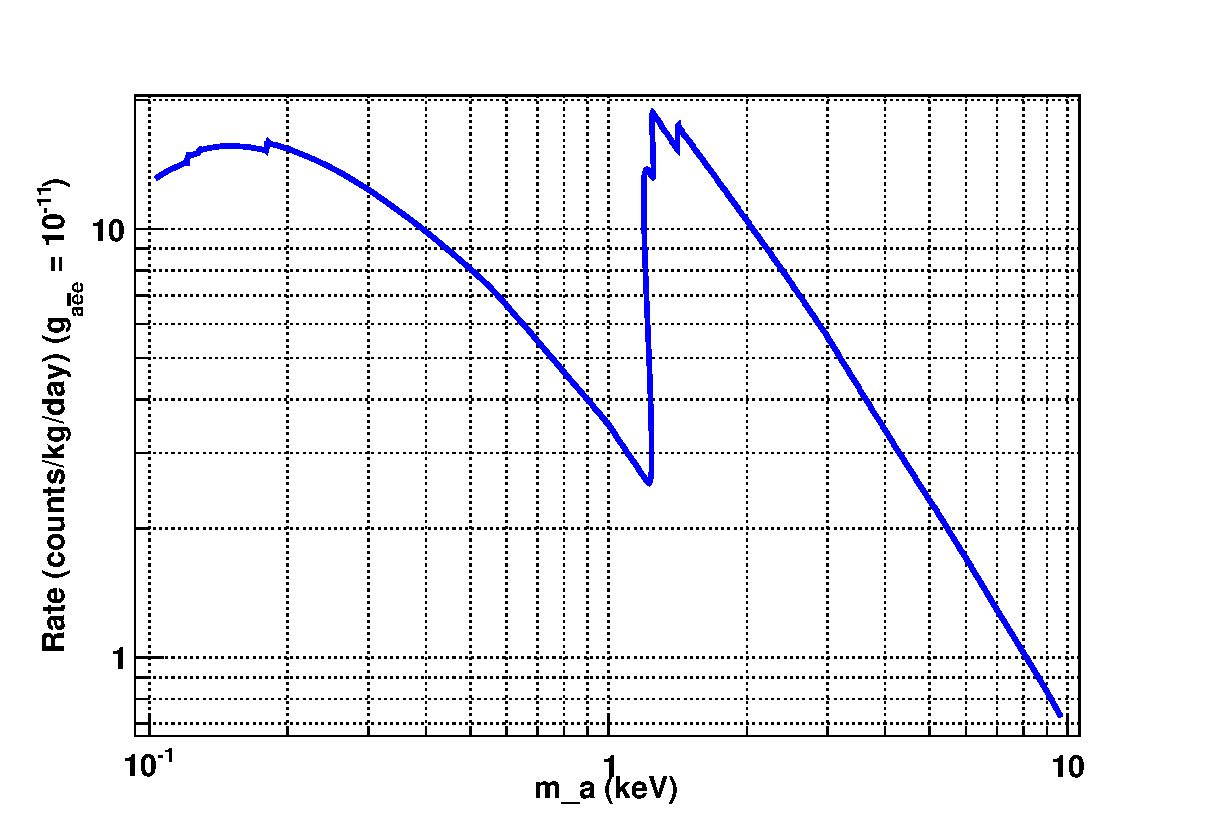
\includegraphics[width=0.9\textwidth]{GeRate}
			\caption[Axioelectric interaction rate in germanium]{Non-relativistic axion axioelectric 
			interaction rate in germanium.  The photoelectric cross section for germanium was obtain
			from the NIST database~\cite{chantler:597}.}
			\label{fig:HeavyAxionSignalRate}
		\end{figure}

	\subsection{Limits on the axioelectric effect}
	\label{sec:CalcLimitsOnHeavyAxionLimits}		
		
	Limits were calculated using the profile-likelihood method described in Section~\ref{sec:LimitsML}.  Fits were performed on the complete number of data sets described in Chapter~\ref{chap:AnalysisBeGe}, with a total live-time of 150.6~days.  All data sets yielded similar results and so one data set was chosen with 95\% rise-time acceptance cuts and microphonics cuts applied.  As outlined before, assumptions about the source of slow-rise-time events reduced the fiducial mass to 0.33~kg (see Section~\ref{sec:BeGeLowEnergyFeatures}).  Additionally, results with unbinned and binned maximum-likelihood fits were consistent and so the former was used for the final result.  The limit calculation followed the same procedure as a peak search in the data and is outlined as follows:
		\begin{itemize}
			\item Define the gaussian signal $f_{axion}$: 
			\begin{itemize}
				\item Choose mass $m_{a}$ of the axion defining $\mu$ of gaussian
				\item Determine $\sigma$ at $E = m_{a}$ using resolution in Equation~\ref{eqn:SigmaEqn}.
			\end{itemize}
			\item Fit to the function $B + N_{axion} f_{axion}$ where $B$ is the background defined in Section~\ref{sec:LimitsDataAndModel} and determine the profile likelihood $\plln$.
			\item Determine the 90\% upper limit on $N_{axion}$ using $\plln$.
			\item Repeat for other values of $m_{a}$
		\end{itemize}		
	
	During the fits, the $\mu$ and $\sigma$ of the gaussian signal, $f_{axion}$, were kept fixed and only the amplitude, $N_{axion}$ was kept as a free parameter of the signal.  For the background, the behavior of the parameters was the same as during WIMP exclusion fits (see Section~\ref{sec:LimitsDataAndModel}) and the relative amplitude of the \gersixeight~and \znsixfive~L-lines was kept fixed as described in Section~\ref{sec:LimitsConstrained}.  Fixing this relative amplitude served to minimize the impact of the L-lines in the exclusion fits since a signal centered at 1.1 or 1.3~keV would look exactly like either L-capture line.  The difficulties seen while determining limits on low-mass WIMPs did not appear in these calculations because the signal (gaussian centered at $m_{a}$) was not similar to the background except for the case of the L-lines.  The value of the axion mass was scanned from 0.1~keV to 7.8~keV in steps of 0.2~keV using both high- and low-gain channels: high-gain channel, $0.1\to2.9$~keV; low-gain channel, $3\to7.8$~keV.  The axion mass was allowed to vary below threshold (0.5~keV) because the finite resolution of the detector would allow portions of the expected gaussian signal to be detected above threshold.  An example of an exclusion fit in the high-gain channel is shown in Figure~\ref{fig:ExampleHeavyAxionFit} for $m_{a}=3$~keV.  

		\begin{figure}
			\centering
			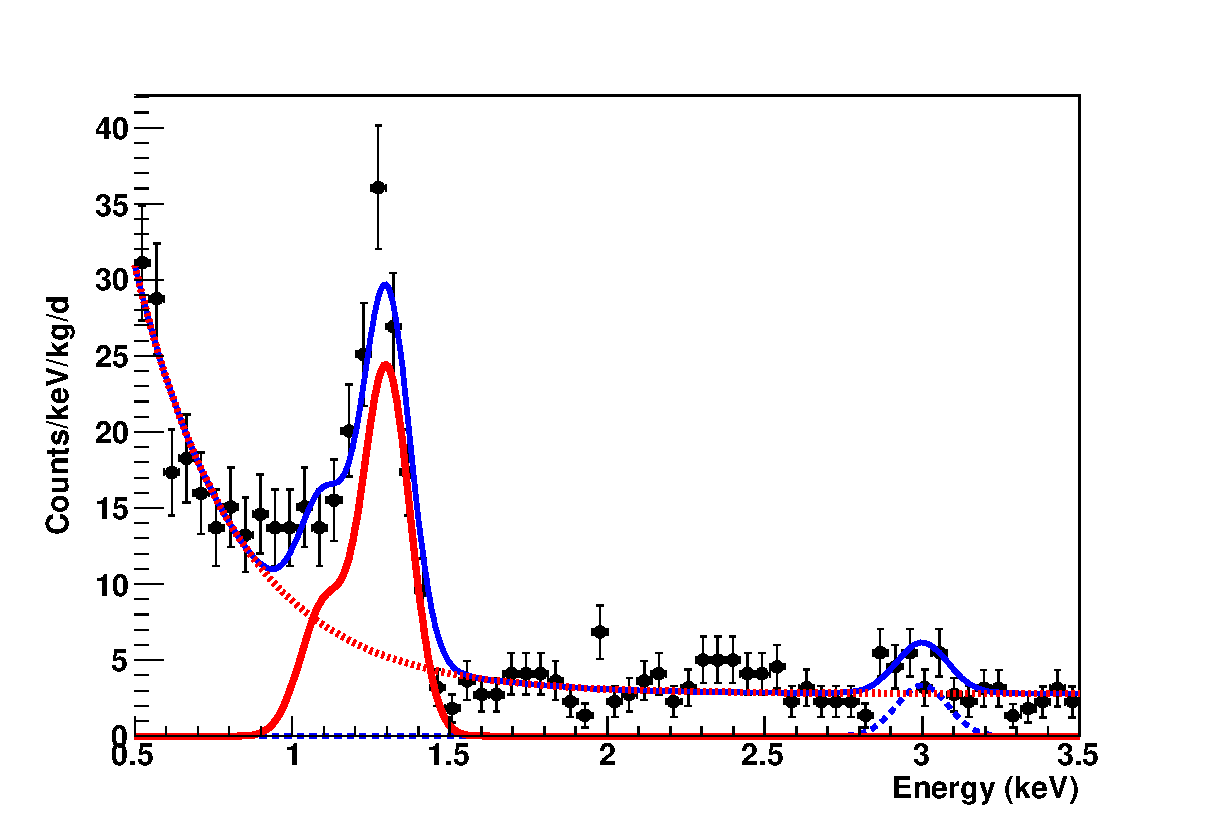
\includegraphics[width=0.9\textwidth]{AxioelectricFitExample}
			\caption[Example of an excluded non-relativistic axioelectric signal at $m_{a}=3$~keV at 
			90\% CL]{Example of an excluded non-relativistic axioelectric signal at $m_{a}=3$~keV at 
			90\% CL.  In this fit performed in the high-gain channel, the excluded value $N_{axion}$ 
			is 36.1 counts.  
			The components of the fits are split: red solid, L-Lines; red dotted, flat plus exponential
			background; blue dashed, excluded axioelectric signal.}
			\label{fig:ExampleHeavyAxionFit}
		\end{figure}
			
	The 90\% CL excluded rate in counts/kg/day, $R_{axion}(m_{a})$, was determined from $N_{axion}$
and from this value the upper limit of $\gaa$ could be determined.  The exclusion calculated from this result is presented in Figure~\ref{fig:HeavyAxionLimits} 
along with a comparison to other results, including previous results of the CoGeNT collaboration~\cite{Aalseth:2008aa}, the CDMS 
collaboration~\cite{Ahmed2009}, and an acceptance region from the DAMA collaboration~\cite{Bernabei:2005ca}.  As noted in both 
references~\cite{Collar:2009sp,Pospelov:2008jk}, the limit calculation performed in~\cite{Bernabei:2005ca} did not correctly treat the 
leading term in the Hamiltonian, producing instead a reduced rate around 3 orders of magnitude lower for a given $\gaa$.  An estimation 
of the corrected result from DAMA as outlined in~\cite{Collar:2009sp} appears in Figure~\ref{fig:HeavyAxionLimits}.  A comparison to 
limits derived from both solar neutrinos~\cite{Gondolo09} and globular clusters~\cite{Raffelt95} is included as well.  

The strongest limits obtained from astronomical observation arise from determining how much `hidden energy' may be carried off by axions from the solar 
core (in the case of solar neutrinos) and similarly from the cooling observed in the evolution of red-giant stars in globular clusters.  All 
direct measurements provide stronger limits than those from solar neutrinos, but the mass-independent limits from globular-cluster 
stars still exceed all others.  Supernovae generally provide the best constraints on axions and other exotic particles, but their high temperatures ($O$(10~MeV)) mean that axion-electron interactions are suppressed according to $m_{e}^{2}/T^{2}$~\cite{Pospelov:2008jk}.  Other limits on pseudoscalars from cosmological observations are possible, including searches for decays to photons and estimates of axion abundance from the big bang.  These limits are discussed with respect to the sensitivity of the \MJ~\minmod~in Section~\ref{sec:MJSensitivityToAxions}.  Even though the presented direct-detection limits are already well within the space disallowed by astronomical constraints, it is still important to explore these parameter regions since limits from both cosmological observation and experiment can depend strongly on choices of models and their parameters.
			
	Pospelov et al.~noted the axioelectric process should be to first order invariant to the velocity of the incoming dark matter particle and so would not generate an appreciable annual modulation.  This would limit any interpretation of the DAMA annual modulation as due to an axioelectric interaction and would therefore disallow the DAMA acceptance region in Figure~\ref{fig:HeavyAxionLimits}.  Collar et al.~point out the possibility of recovering the annual modulation effect by considering the axioelectric interaction rate as not arising from changes in incident dark matter velocity but rather from the annual variation of the number density of the particles~\cite{Collar:2009sp}. 
			
		\begin{figure}
			\centering
			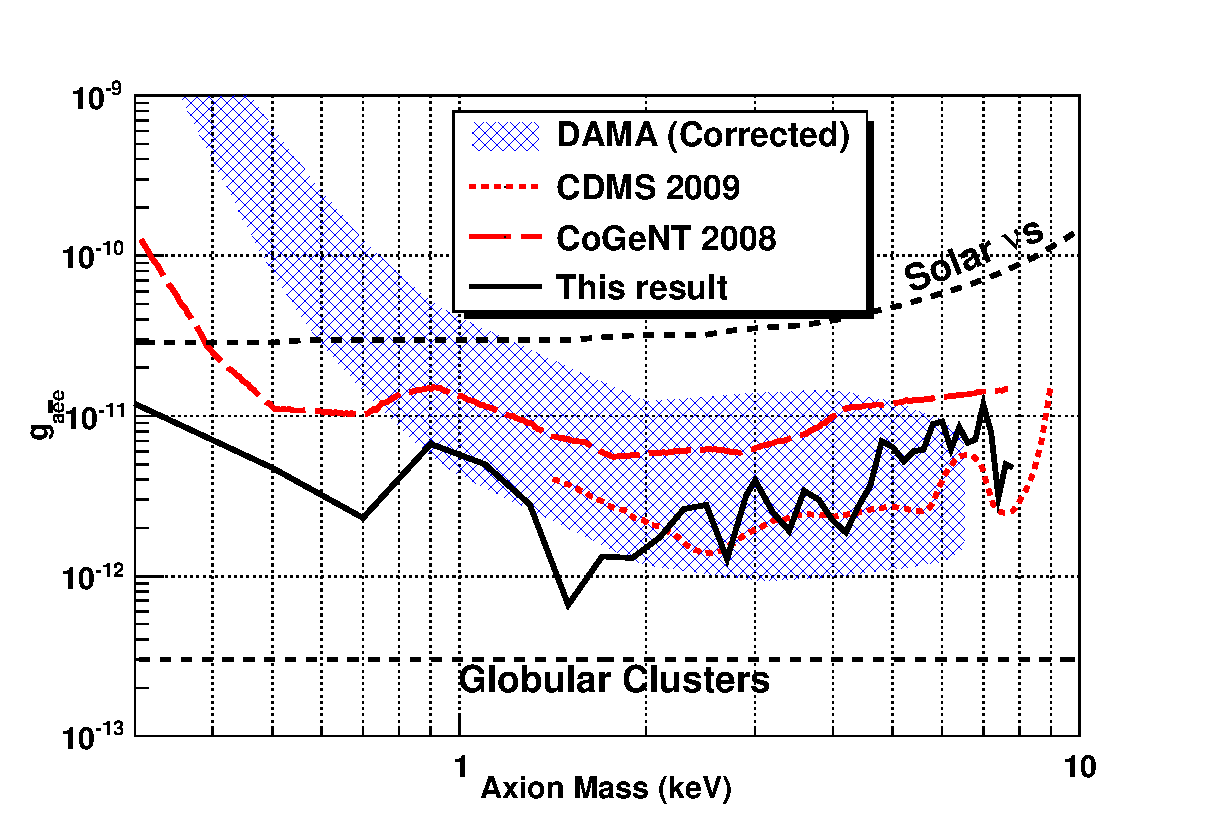
\includegraphics[width=0.9\textwidth]{axion_constrained_unbinnedall_exclusion_plots_final}
			\caption[Limits on the axioelectric coupling constant $\gaa$]{Limits on the axioelectric 
			coupling constant $\gaa$.  Results from this work appear in comparison to previous 
			results from CoGeNT~\cite{Aalseth:2008aa}, CDMS~\cite{Ahmed2009}, and 
			DAMA~\cite{Bernabei:2005ca}.  The DAMA results have been corrected per 
			reference~\cite{Collar:2009sp}.  Limits derived from both solar neutrinos~\cite{Gondolo09} and globular clusters~\cite{Raffelt95} are included as noted, see text for details.}
			\label{fig:HeavyAxionLimits}
		\end{figure}
		
	\subsection{Conclusions and Discussion}
	\label{sec:DiscOnHeavyAxionLimits}	

%	Note what we've done here, in particular looking at an axioelectric signal in data.  Also note that this is one very small detector that's comparable to a large array.  Talk about how this could be better with MJ and how the limits from astrophysical observations still need to be checked.  
	
	The results from this section underscore and emphasize the physics reach of \ppc~detectors.  In particular, a limited amount of data from a small `table-top' detector (mass exposure $\sim50$~kg-days) yielded results comparable to results from CDMS which had more than a factor of 5 greater exposure time (443.2~kg-days).  
% FixME JFW: Make above sentence more diplomatic	
Though limits derived from astronomical observations still exceed those from direct-detection experiments, it remains important to verify these limits and, if possible, better them with larger exposure times and smaller backgrounds.  The need to explore dark matter candidates beyond those offered by WIMP theories remains evident and the only method to ensure experimental sensitivity to rare events with an \emph{a priori} unknown signature is to reduce known backgrounds through appropriate shielding and detector component radio-purity.  The \MJ~experiment seeks to do this to search for $\nonubb$, but the same efforts to reduce backgrounds in the double-beta decay signal region ($\sim2$~MeV) should benefit searches for dark matter in low-energy regions.  The following sections discuss and calculate the sensitivity of the \MJ~\minmod~for such searches.
							
	\section{Sensitivity of the \MJ~\minmod~to dark matter signals}
	\label{sec:MJSensitivity}
	
	Since a framework was established to determine exclusion limits for low-mass WIMPs and for the axioelectric coupling constant, it is simple to apply this same framework to determine the sensitivities of the \MJ~\minmod~to these two dark matter signals.  The ultra-clean composition of the \minmod~should provide an excellent detector for searching for dark matter without relying upon significant background reduction cuts (e.g.~discrimination between nuclear and electron recoils).  Calculating the sensitivity of the experiment involves making some assumptions of the background at low energies and of the makeup of the experiment.  A discussion about the estimation of the background follows in Section~\ref{sec:MJLowEnergyBackgroundModel}.  The general prescription for calculating the sensitivity is outlined:
	
		\begin{itemize}
			\item Generate a background model, including an expected rate of background
			\item Simulate a spectrum according to the background model
			\item Fit to the simulated spectrum the background model plus a signal model (e.g.~WIMP or axioelectric spectrum)
			\item Calculate the upper limit on the amplitude of the signal at 90\% CL.
			\item Repeat a large number of times ($O$(1000)) to generate an ensemble of limits.
		\end{itemize}	
		
The generated ensemble of limits for a particular signal would create a distribution of limits.  The 90\% CL limit was chosen as the limit which was above 99\% of the entries in this distribution.  Details of the \MJ~\minmod~are given in Section~\ref{sec:MJExperiment}, but for these purposes we have conservatively assumed that the \MJ~\minmod~will be composed of 20~kg of material and that it will accumulate between 1 and 5~years of live-time.  
	
		\subsection{Low-energy background model}
		\label{sec:MJLowEnergyBackgroundModel}
		
The estimation of background generally comes from verified simulations and from extrapolations from previous experiments.  In this work, the background is estimated by assuming it arises from two main sources: (1) a continuum from higher energy processes, and (2) counts from the beta decay of cosmogenically-produced tritium in the detector.  A simulation to estimate (1) is wrought with challenges since a large number of contributions can affect the result.  However, it is possible to use previous results from low-background germanium-based experiments to produce an estimate of this background.  The IGEX experiment measured a flat background rate of $\sim0.1$~counts/keV/kg/day in this low energy region ($4\to10$~keV)~\cite{Ira01}.    The \MJ~\minmod~plans to reduce background above 200~keV by a factor of 100~\cite{Gaitskell:2003zr} and so it is reasonable to expect the flat background at low energies will follow this same reduction to be roughly 0.001~counts/keV/kg/day.  This background was assumed stable in time as well, so that it was flat in both time and energy.

The estimate of a background to tritium involves understanding the activation rate of tritium for germanium at the surface of the earth.  This activation rate has been estimated to be $\lesssim200$~\hthree-atoms-per-kilogram-of-Ge-per-day for natural germanium at the surface of the earth, and almost a factor of 2 less for germanium with enriched \gersevensix~content~\cite{Avi92}.  Other references have suggested that this rate is roughly an order of magnitude too high~\cite{Col92,Mei:2009vn}; we conservatively use the enhanced rate, but assuming a smaller activation would correspondingly lengthen an allowed exposure time.  The exposure is determined by the time of manufacture beginning with the pulling of the germanium crystal and ending when the crystal is brought underground.  For example, if the entire process from crystal pulling to detector development and then final deployment (or storage) underground takes 15~days, then this integrated time is the the total tritium activation period for the detector.  For a kilogram natural-germanium detector created over such a time scale, we would expect there to be $15\times200\sim3000$ atoms of \hthree~within the detector.  Given the slow time of decay of \hthree~(12.32~years), it is critical to minimize the time above ground and certainly necessary to avoid any time at high altitudes, e.g.~storage or transport via airplane.  In this simple background model, two optimistic exposure times are chosen -- 15 and 30~days -- and it is assumed that the detectors begin taking data immediately after arriving underground.  In practice, the assumption of immediate detector commissioning is justified due to the long decay time of tritium: the detector will not significantly cool down during a period of time underground much shorter than the tritium lifetime.  The average rates due to these exposures once underground are then roughly 0.03 and 0.06~counts/keV/kg/day for 15 and 30~days, respectively.  

The pdf of the tritium decay function was constructed in both time and energy using the corrected kinematic equation:
		\begin{equation}
			f_{^{3}\text{H}}\left(E, t\right)  =  g_{^{3}\text{H}}\left(E\right) \times h_{^{3}\text{H}}\left(t\right) 
		\end{equation}
		with
		\begin{eqnarray}
		g_{^{3}\text{H}}\left(E\right) & = & \sqrt{(E + M_e)^2 - M_e^2} \left(
			E + M_e \right) \left( Q_{^3\text{H}} - E \right)^2 F(Z, E) \\
h_{^{3}\text{H}}\left(t\right) & = & e^{-t/\tau_{^3\text{H}}} \\
		F(Z,E) & =  & y ( 1 - e^{-y} )^{-1} (1.002037 - 0.001427(v/c)) \\
		y & = & \frac{2 \pi Z \alpha}{v/c} \\
		\end{eqnarray}
		where $F(Z,E)$ is an approximation of the screened and relativistic Fermi function with $Z = 2$ for the daughter nucleus (as determined by J.~J.~Simpson in~\cite{Simp81}) and $Q_{^3\text{H}}=18.6$~keV, $M_{e}=511$~keV, and $\tau_{^3\text{H}} = 12.32 / \log(2)$~years.  
		
	The background from neutrons has been estimated previously for the IGEX experiment~\cite{Carmona2004523} located at the Canfranc underground laboratory.  This reference considered both neutrons from cosmic-ray muons interacting in the rock as well as neutrons arising from spontaneous fission and ($\alpha$, n) reactions.  Estimates from this -- see Figure~7 and Tables 2,3 in~\cite{Carmona2004523}, Figure~7 reproduced here in Figure~\ref{fig:IGEXNeutrons} -- suggested that contributions to IGEX from both sources should be below 0.01~counts/keV/kg/day down to 0~keV.  Additionally, it was demonstrated that neutrons from rock radioactivity could be effectively eliminated with additional shielding.  Though the \MJ~\minmod~will have a different geometry to that of the IGEX experiment, it is expected that these numbers are a conservative upper limit due to the fact that the \minmod~will be in a deeper location (DUSEL ($\lesssim4500$~m.w.e.) vs.~Canfranc (2500~m.w.e.)).  From these conclusions and because the background from \hthree~should at least initially dominate the \minmod, any background contribution from neutrons was omitted from the background model.
	
			\begin{figure}
				\centering
				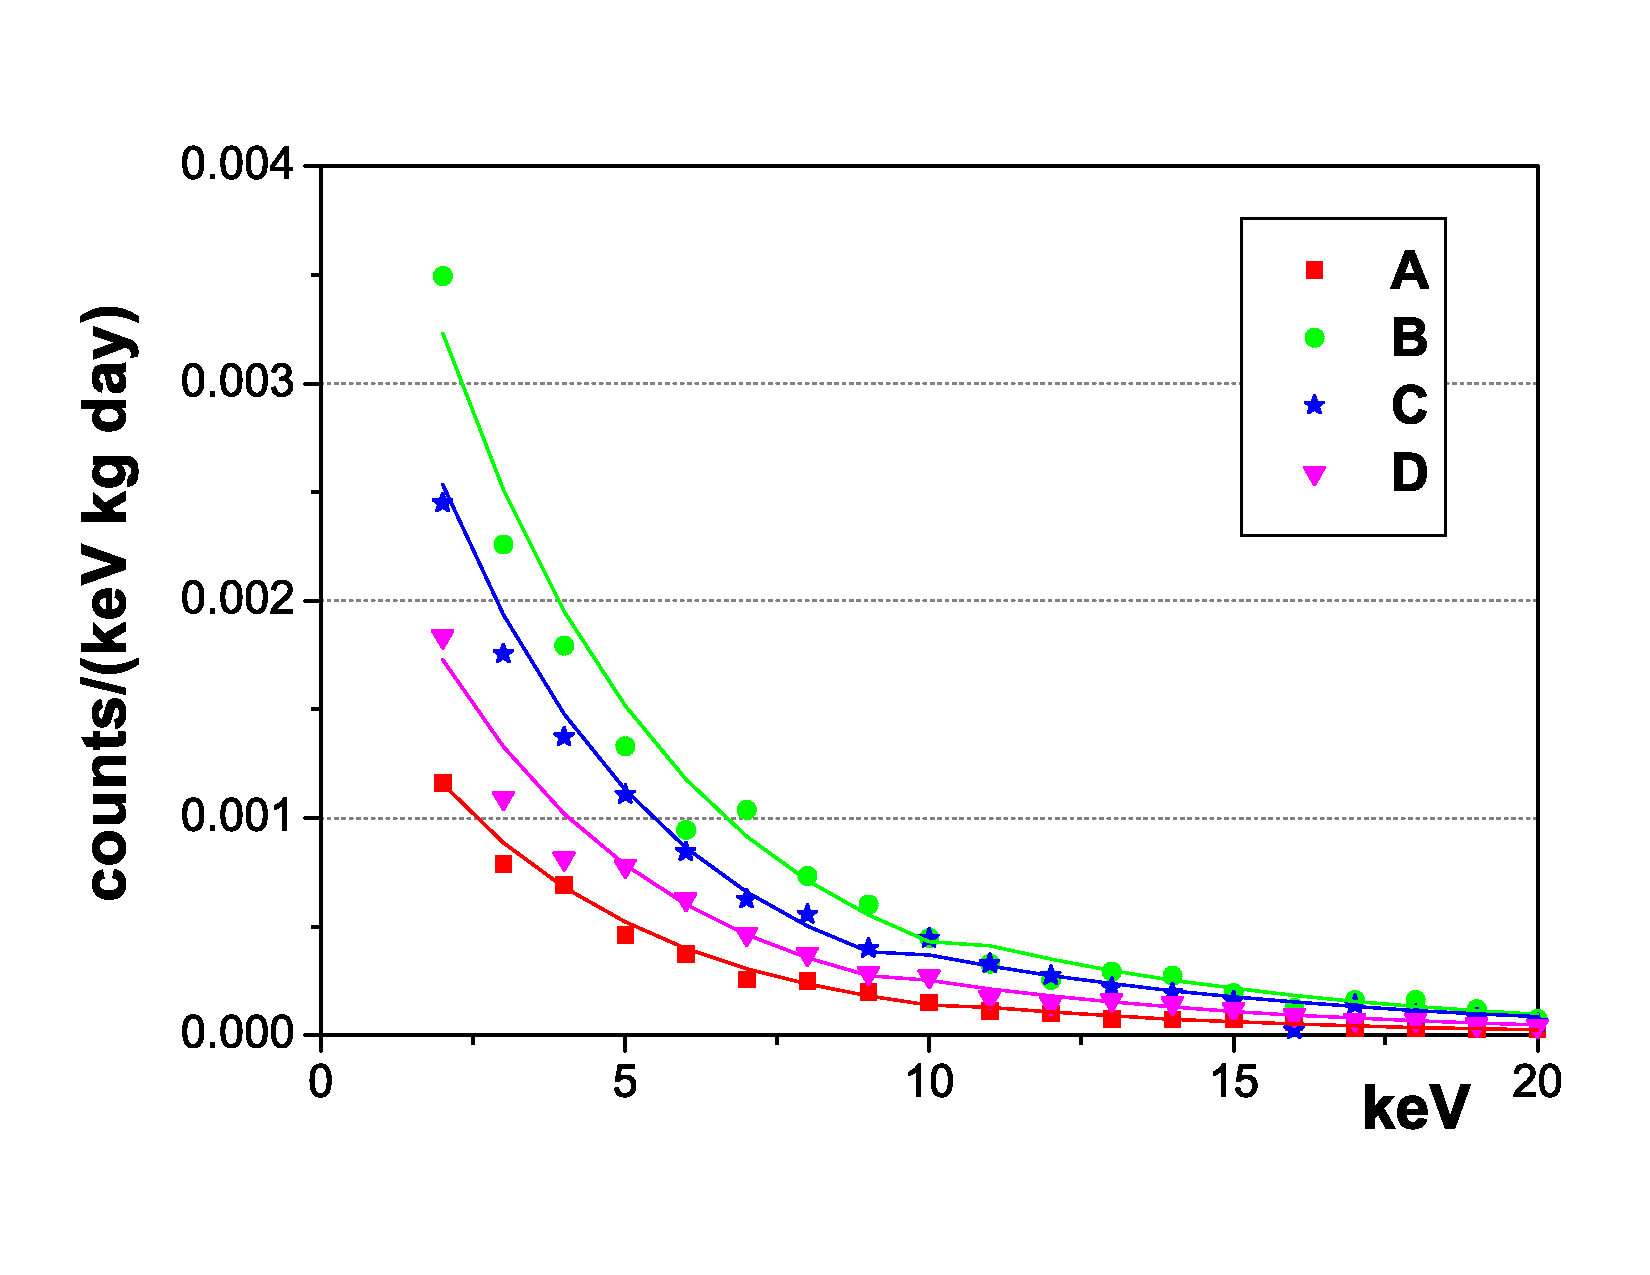
\includegraphics[width=0.9\textwidth]{IGEXNeutronsFromMuons}
				\caption[Simulated muon-induced-neutron spectrum for IGEX.]{Simulated muon-induced-neutron 
				spectrum for IGEX, reproduced from Figure~7 in reference~\cite{Carmona2004523}.  A, B, C, and D are different
				neutron moderator configurations for the IGEX experiment, and the lines are exponential fits to guide the eye.
				A conservative extrapolation suggests that the smallest of these spectra (A) 
				should be well below 0.01~counts/keV/kg/day at
				0.5~keV and that all the spectra are much less than 0.001~counts/keV/kg/day above 10~keV.}
				\label{fig:IGEXNeutrons}
			\end{figure}
	
	In general, the detector response must be convolved with the spectrum to get a realistic shape.  However, since point-contact detectors have such excellent energy resolution ($\sigma\sim70$~eV), the response has limited effect on the spectra.  Therefore, no correction for finite resolution was taken into account.  

		\subsection{Sensitivity Fitting}
		\label{sec:MJSensitivityFitting}
	
	The fitting procedure used binned maximum likelihood instead of an unbinned fit to reduce the time required in estimating an upper limit for each toy data model.  Three parameters affecting the fits were varied: tritium exposure time, threshold, and exposure time of the \minmod.  Each of these parameters could take two different values (see Table~\ref{tab:SensFitValues}) so that for each signal eight different sets of fits were done.  The data sets and fitting PDFs were both fully two-dimensional in energy and time and were fit over a range from threshold to 20~keV.  The binning was chosen as follows: 256~bins for energy and 16~bins for time.  For each of the eight set of fits for a signal, an ensemble of upper limits with a population $\gtrsim1500$\footnote{ An exact population number was not specified for the ensembles to maximize the efficiency of the calculation.  It was more efficient to specify the \emph{time} for the calculation to run than to define a specific number of iterations.} was generated on the Athena cluster at the University of Washington~\cite{Athena}.  The final sensitivity calculations outlined in the following sections took roughly 1500~hours of real-time or 460~cpu-days.
	
			\begin{table}
				\centering
				\begin{tabular}{l r}
					\toprule
					Variable & Values \\
					\midrule
					\hthree~exposure time & 15, 30~days \\
					Threshold & 0.3, 0.5~keV \\
					\minmod~exposure & 1, 5~years (20, 100~kg-years) \\
					\bottomrule 
				\end{tabular}				
				\caption[Variations on background and fitting for \MJ~\minmod~sensitivity calculations]
				{Variations on background and fitting for \MJ~\minmod~sensitivity calculations}
				\label{tab:SensFitValues}
			\end{table}		
		
		\subsection{Sensitivity to WIMPs}
		\label{sec:MJSensitivityToWIMP}
		
	The sensitivity calculations for WIMPs employed the 2-dimensional (time, energy) signal described in the previous chapter; more details can be found in Section~\ref{sec:CalcLimitsOnWIMPSignal}.  The values for all constants in the WIMP signal were used as previously noted.  The fits proceeded as outlined in the previous section (Section~\ref{sec:MJSensitivityFitting}).  The shape of the WIMP signal was parameterized solely by the mass of the WIMP, $M_{W}$, and so fits were performed with different values of this parameter on a variable grid (in GeV) of spacing given in $\Delta M_{W}$, $M_{W}=$ 2.9; 3; 3.5; $4\to10, \Delta M_{W} = 1$; $12\to24, \Delta M_{W} = 2$; $30\to100, \Delta M_{W} = 10$; $100\to1000, \Delta M_{W} = 100$.  An example sensitivity fit to a WIMP signal at $M_{W}=10$~GeV is given in Figure~\ref{fig:MJSensitivityToWIMPExample}.  In this particular example, the threshold was 0.3~keV, \hthree~exposure time was 15~days, and the total exposure time was 1~year.  It is clear that the amplitude of the excluded signal is very small and perhaps smaller than one might expect given the average count rate dominated by the \hthree~decay.  However, the shape of a WIMP signal is significantly different from that of a tritium beta spectrum making a stronger exclusion possible because the shape of the spectra are taken into account.  A simple integration analysis looking solely at counts in a defined energy window should not produce the same limits.  
		
			\begin{figure}
				\centering
				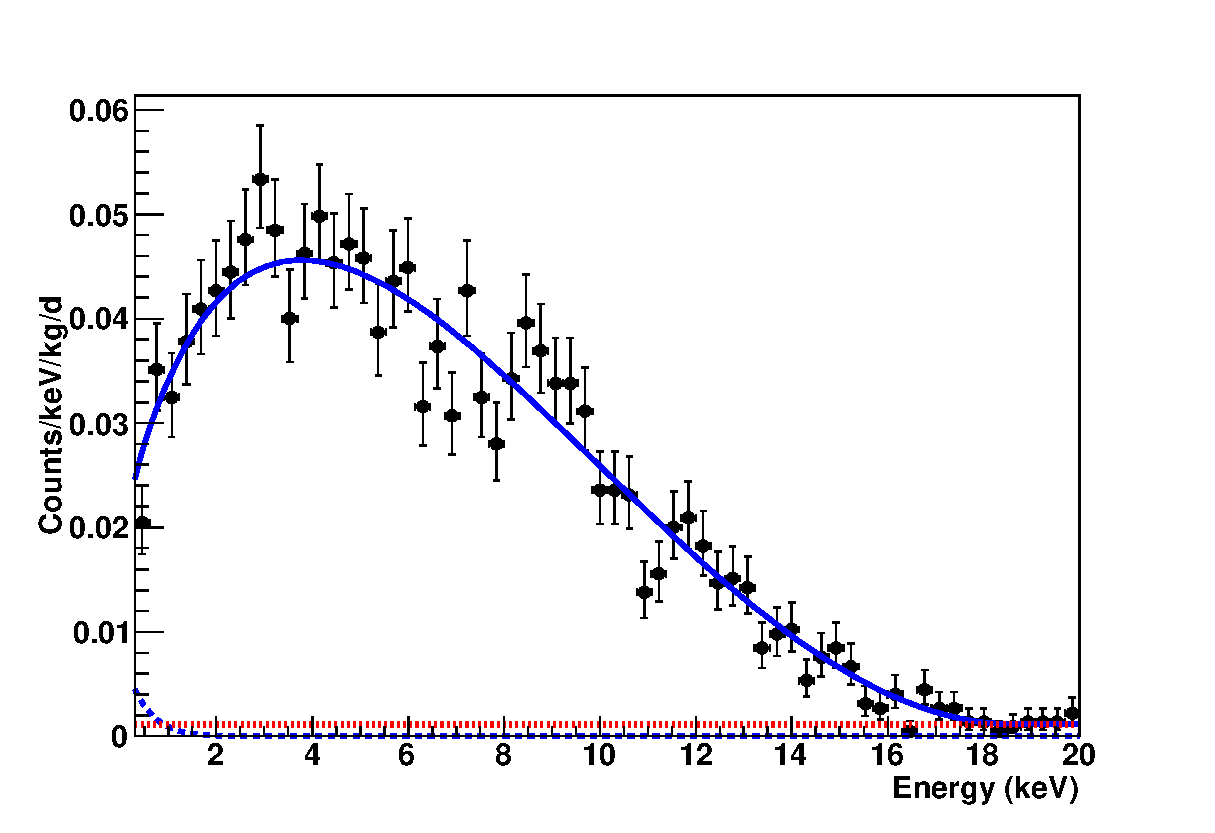
\includegraphics[width=0.9\textwidth]{MJDemoExampleSensFit}
				\caption[\MJ~\minmod WIMP sensitivity fit example.]{A sensitivity fit example with WIMP  
				signal at $M_{W}=10$~GeV, with $\signuc$ excluded at 90\% CL with value
				 $8.6\times10^{-9}$~pb.  Components of the fit are broken out including WIMP 
				 signal (blue dashed) and flat background (red dotted).  The beta spectrum from \hthree~dominates the fit.}
				\label{fig:MJSensitivityToWIMPExample}
			\end{figure}
	
	The final results of the sensitivity calculation are presented in Figure~\ref{fig:MJSensitivityToWIMP}.  This figure includes results from the eight different sets of fits with the modification of the exposure times and the threshold.  The factor of 2 increase in exposure time doesn't have a significant impact other than softening the exclusion limits as the WIMP mass increases.  The threshold has a fairly significant impact below 10.5~GeV yielding better exclusions for WIMP masses and pushing the exclusion region diagonally left and down in the plot.  This is certainly due to the sharp reduction of the tritium spectrum at low energies and to the sharp turn on of the exponential-like WIMP spectrum.  As expected, the reduced threshold of 0.3~keV enables limits to be made down to $M_{W}=3.5$~GeV.  
	
			\begin{figure}
				\centering
				\def\figheight{0.41\textheight}				
				\subfigure[1~year (20 kg-yr) exposure time]{
					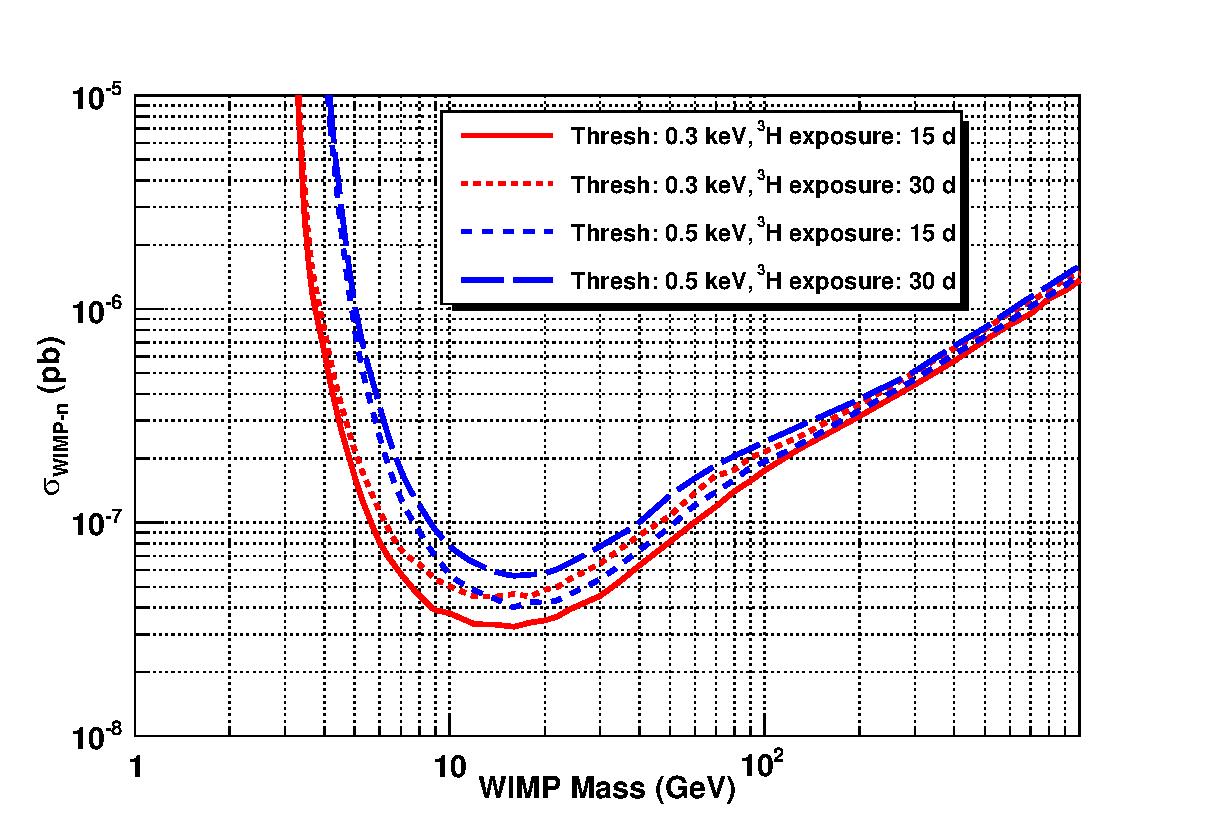
\includegraphics[height=\figheight]{20TimeExposureMJ}
					\label{fig:20TimeExposureMJ}						
				}
				\subfigure[5~year (100 kg-yr) exposure time]{
					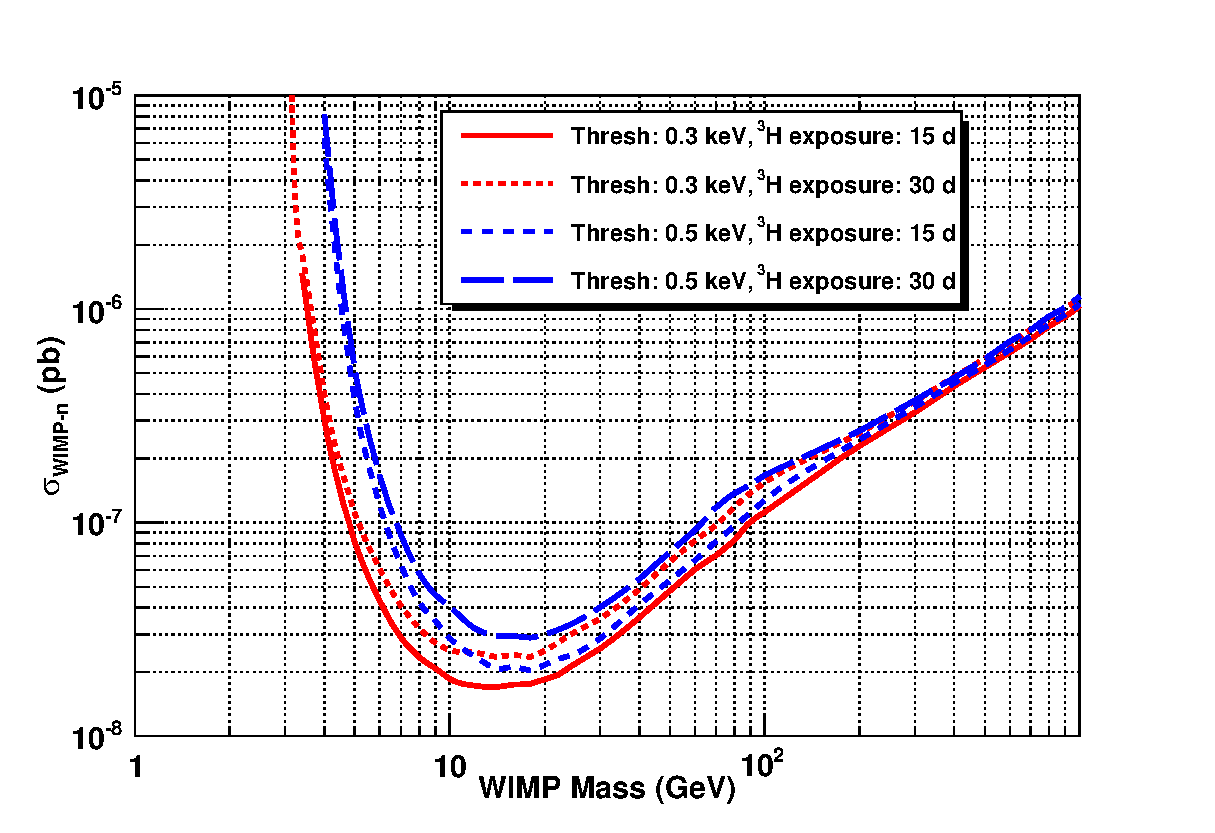
\includegraphics[height=\figheight]{100TimeExposureMJ}
					\label{fig:100TimeExposureMJ}						
				}				
				\caption[\MJ~\minmod~sensitivity to a WIMP signal]{\MJ~\minmod~sensitivity.  Lines are 90\% confidence level exclusions.}
				\label{fig:MJSensitivityToWIMP}
			\end{figure}		
	
	It is instructive to compare the estimated sensitivity of the \minmod~to that of other WIMP dark matter experiments.  The \MJ~experiment is distinct from most dark matter experiments since, for one, it is not primarily seeking to detect dark matter, but also because it will not rely upon any significant background reduction technique to enhance its sensitivity to WIMP-induced nuclear recoils.  That is, the \MJ~experiment will not have the ability to distinguish between nuclear and electron recoils.  Despite this, it can still be competitive because it can access parameter space unreachable by other experiments with higher thresholds.  A comparison of the sensitivity of the \MJ~\minmod~(assuming 0.3~keV threshold, 15~day tritium exposure, and 100~kg-yr exposure) to two characteristic dark matter experiments is given in Figure~\ref{fig:MJSensitivityToWIMPCompare}.  These two experiments include Phase A of SuperCDMS~\cite{Akerib2006411} and the 300~kg LUX experiment~\cite{LUX300}.  The former is a proposed Ge-based dual-mode bolometer and ionization detector, the latter a proposed liquid-Xe-based detector that would read out both scintillation light and ionization.  The dual-mode nature of these detectors gives them the ability to tag nuclear recoils and reject the electron recoils which dominate the background spectrum.  Whereas it is obvious that the reach of these experiments in the higher-WIMP-mass range ($>10.5$~GeV) far exceeds that of the \MJ~\minmod, the low-energy threshold of the \minmod~enables it to push well into the lower-WIMP-mass region.  
		
			\begin{figure}
				\centering
				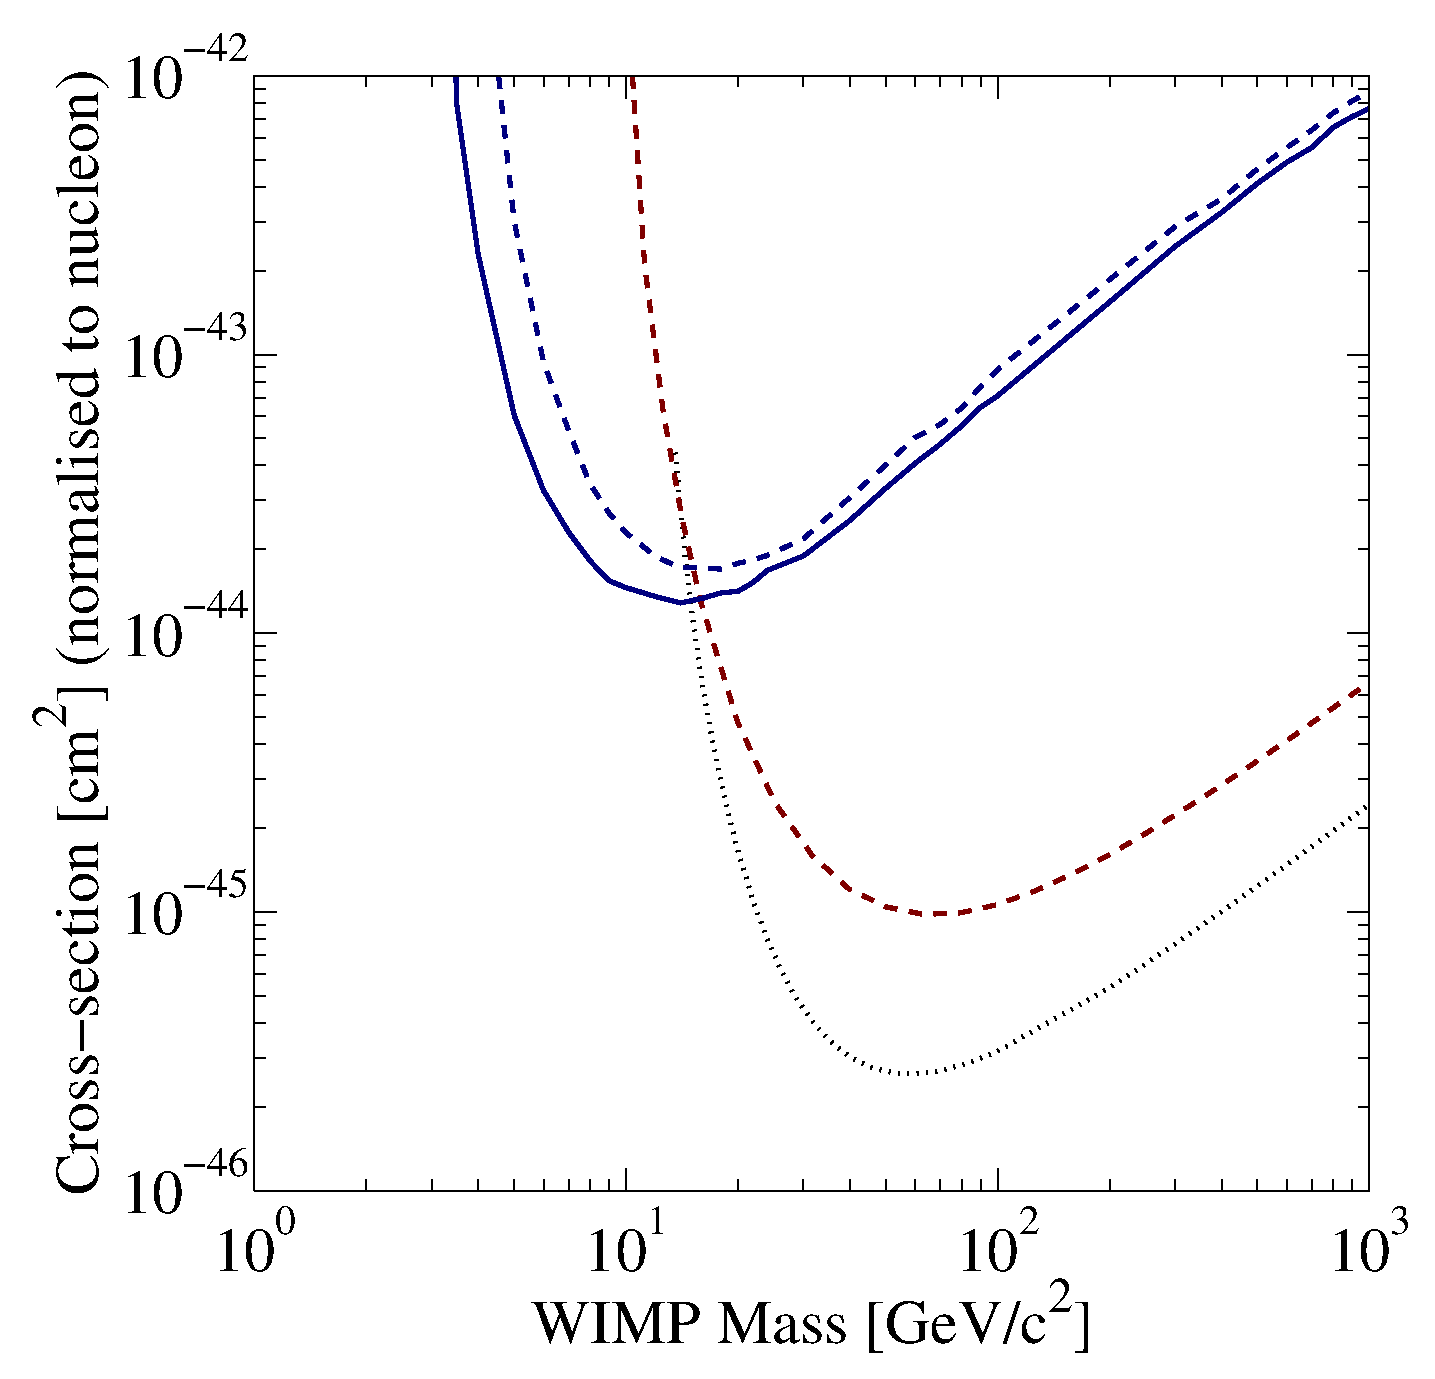
\includegraphics[width=0.9\textwidth]{MGM_MJ_Sensitivity_Compare}
				% FixME JFW: explain MJD more than one line.
				% Also FixME: get new plot from DMTools
				\caption[\MJ~\minmod~sensitivity to a WIMP signal, comparing to SuperCDMS Phase A and LUX 300.]
				{\MJ~\minmod~sensitivity to a WIMP signal (blue solid), comparing to SuperCDMS Phase A~\cite{Akerib2006411}(red dashed) and LUX 300~\cite{LUX300}
				(black dotted).  Plot generated with DMTools~\cite{Gai03}, lines are 90\% CL exclusions.}
				\label{fig:MJSensitivityToWIMPCompare}
			\end{figure}			
			
		\subsection{Sensitivity to axioelectric effect}
		\label{sec:MJSensitivityToAxions}
		
	The sensitivity calculations for the axioelectric effect employed the signal model outlined earlier in Section~\ref{sec:CalcLimitsOnHeavyAxionSignal}.  For simplicity and because it is expected that the rate of interaction does not vary significantly in time~\cite{Pospelov:2008jk}, this model was only 1-dimensional in energy.  The mass of the axion, $m_{a}$, was chosen on a variable grid (in keV) with spacing given in $\Delta m_{a}$: $0.1\to1, \Delta m_{a} = 0.1$; $1\to9, \Delta m_{a} = 0.2$.  An example sensitivity fit to an axioelectric signal centered at $m_{a}=5$~keV is shown in Figure~\ref{fig:MJSensitivityToAxionExample}.  In this example fit, a threshold of 0.3~keV and and a tritium exposure time of 15 days is assumed.  As before, components of the fit appear separately for comparison.   
		
			\begin{figure}
				\centering
				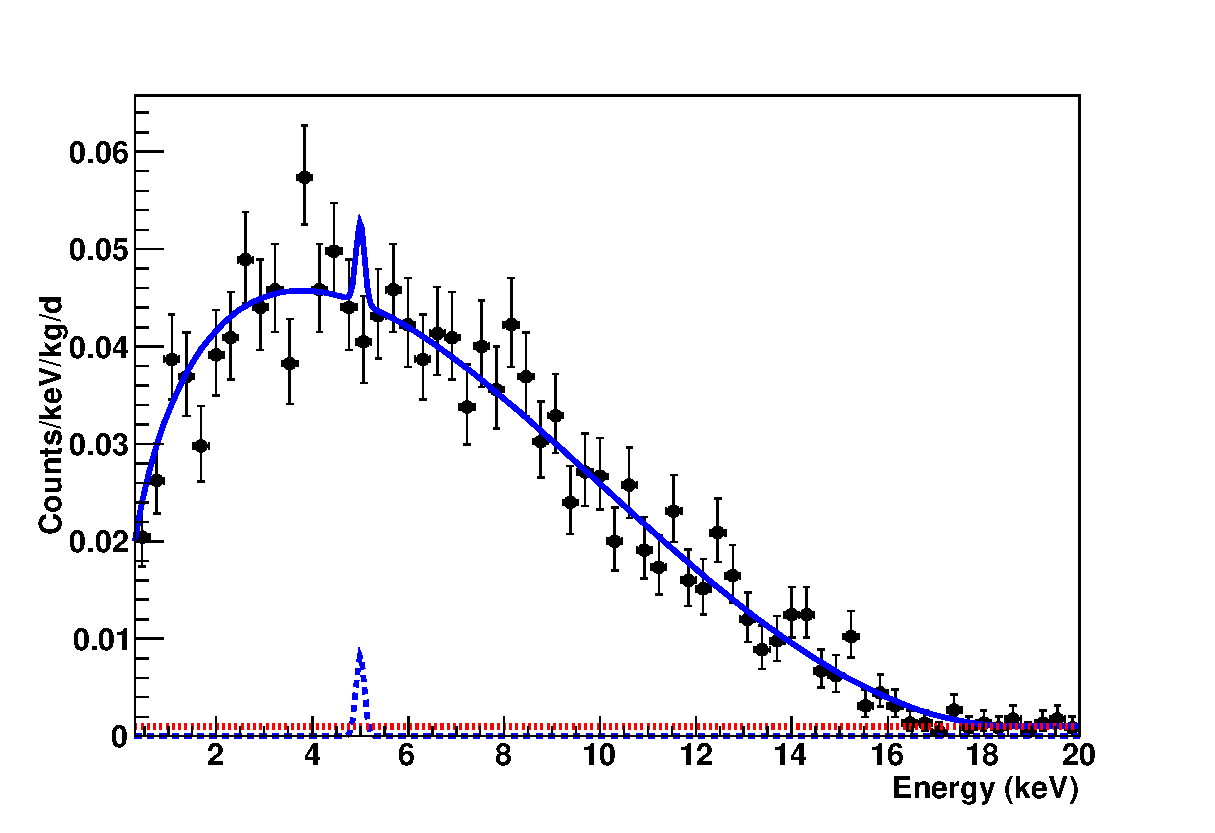
\includegraphics[width=0.9\textwidth]{MJDemoExampleSensFitAxion}
				\caption[\MJ~\minmod axioelectric sensitivity fit example.]{A sensitivity fit example 
				with axioelectric signal at $m_{a}=5$~keV, with $\gaa$ excluded at 90\% CL with
				value
				 $4.4\times10^{-11}$~pb.  Components of the fit are broken out including axioelectric 
				 signal (blue dashed) and flat background (red dotted).  }
				\label{fig:MJSensitivityToAxionExample}
			\end{figure}
	
	The sensitivity for the \MJ~\minmod~to the axioelectric effect is presented in Figure~\ref{fig:MJSensitivityToAxion}.  All of the exclusion plots have similar characteristics, including a sharp drop at $m_{a}=1.3$~keV and a rise at low $m_{a}$.  The former arises from the corresponding feature in the rate (Figure~\ref{fig:HeavyAxionSignalRate}) due to the L-capture line resonance.  The latter comes as the signal moves below threshold and the `leakage' of signal from lower energies pushes above threshold due to the finite energy resolution of the detector.  Larger tritium exposure time softens the sensitivity, but not significantly because $\gaa$ appears squared in the rate equation (Equation~\ref{eqn:AxioelectricRate}).  Also, as expected at higher $m_{a}$ the sensitivity has no dependence on the threshold.
	
			\begin{figure}
				\centering
				\def\figheight{0.41\textheight}
				\subfigure[1~year (20 kg-yr) exposure time]{
					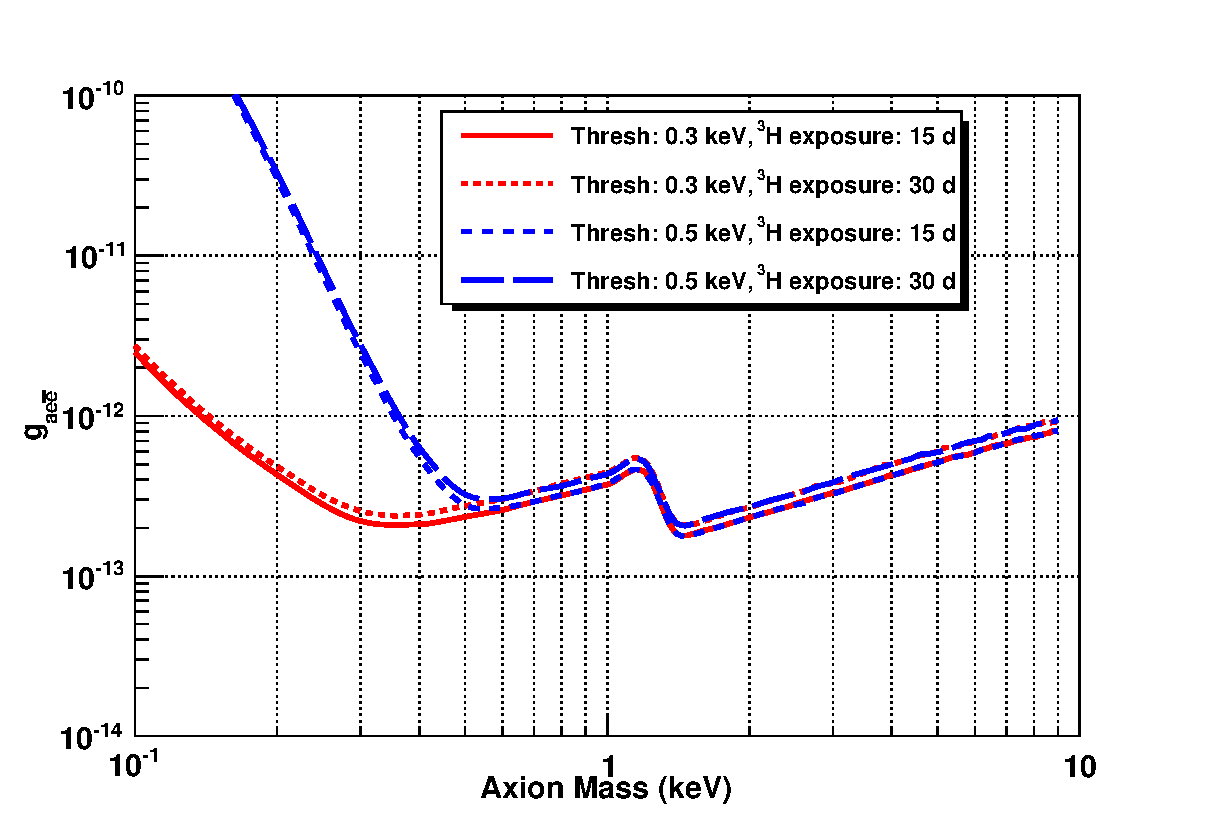
\includegraphics[height=\figheight]{1TimeExposureMJAxion}
					\label{fig:20TimeExposureMJAxion}						
				}
				\subfigure[5~year (100 kg-yr) exposure time]{
					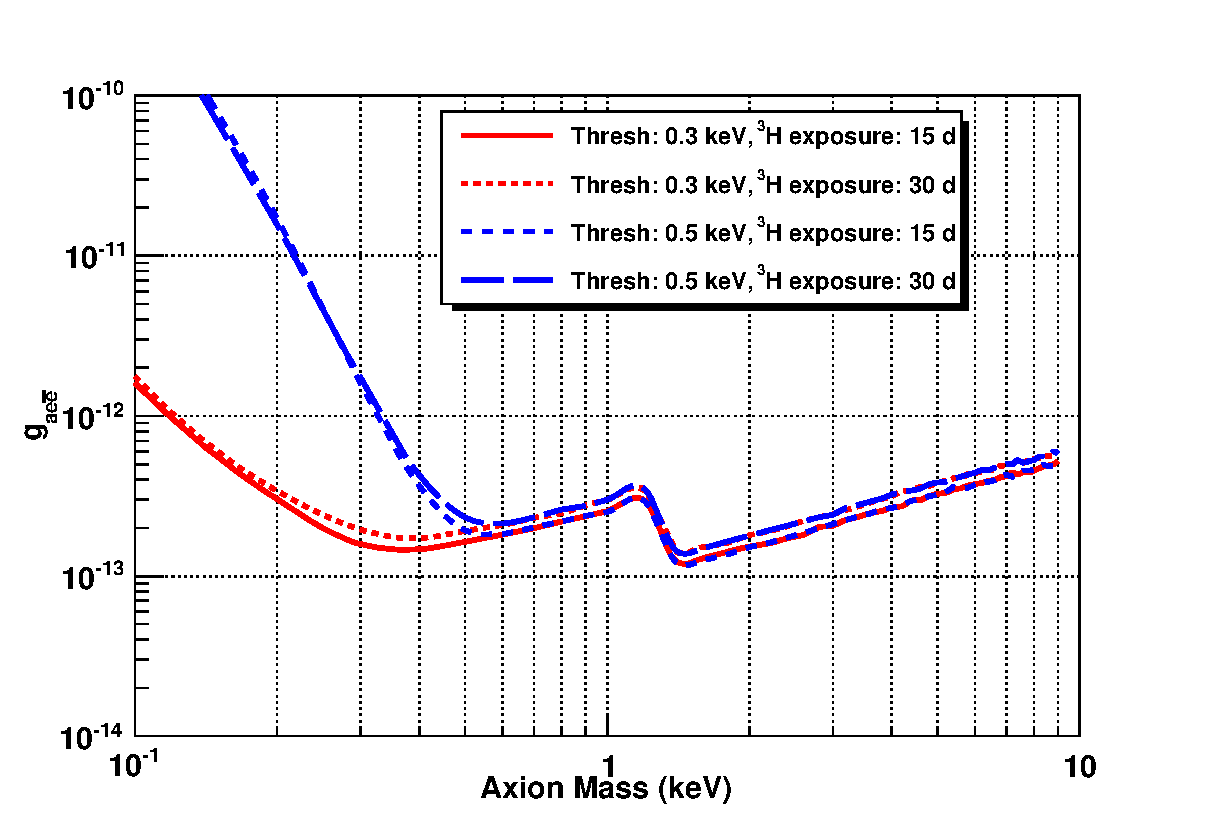
\includegraphics[height=\figheight]{5TimeExposureMJAxion}
					\label{fig:100TimeExposureMJAxion}						
				}				
				\caption[\MJ~\minmod~sensitivity at 90\% CL to an axioelectric signal]{
				\MJ~\minmod~sensitivity at 90\% CL to an axioelectric signal.  Exposure time for \hthree~and threshold were varied and results displayed as noted
				in the figure legends.}
				\label{fig:MJSensitivityToAxion}
			\end{figure}	
				
	%A comparison plot to other experiments has not been generated because no experiments have published sensitivities to the axioelectric effect.  However, since most other dark matter experiments rely upon background reduction through electron and nuclear recoil discrimination, it is possible that these experiments will not have a significant sensitivity to an axioelectric signal because the process appears as an electron recoil event.  
	To help compare with results presented before in Figure~\ref{fig:HeavyAxionLimits}, Figure~\ref{fig:MJSensitivityToHeavyAxionsCompare} is shown including exclusion limits from %solar neutrinos~\cite{Gondolo09} and 
	globular clusters~\cite{Raffelt95}.  Additional limit estimates from~\cite{Pospelov:2008jk} are included, in particular those from searching for decays of exotic particles to photons and for big bang dark matter abundance considerations.  For the first limit, the lifetime of the decay of the axion to 2 photons is given by (see~\cite{Pospelov:2008jk}):
	
			\begin{equation}
				\Gamma_{a \to 2 \gamma} = \frac{C_\gamma}{4 \pi f_a^2} m_a^3
			\end{equation}
with
			\begin{equation}
				C_\gamma \sim \frac{\alpha}{\pi} \frac{m_{a}^{2}}{m_{e}^{2}}
			\end{equation}
Following~\cite{Pospelov:2008jk} and references therein, evidence from astronomical searches for monochromatic photons puts a limit in the 10~keV region of $\Gamma_{a \to 2 \gamma} < 10^{-27} s^{-1}$ which yields an expected exclusion of 
			\begin{equation}
				\gaa < 10^{-11} \left(\frac{\text{keV}}{m_{a}}\right)^{7/2}
			\end{equation}
As well, Pospelov et al.~considered abundance limits on dark matter axions generated from $b$-quarks after the big bang, estimating that 
			\begin{equation}
				\gaa < 10^{-13} \sqrt{
					\left( 2 \frac{\Omega_a}{\Omega_{\text{baryon}}} \right)
					\left( \frac{\text{keV}}{m_a}\right)
				}
			\end{equation}
where $\Omega_{a}$ is estimated as $\Omega_{DM}$ so that $\Omega_a/\Omega_{\text{baryon}} \sim 10$ and therefore:
			\begin{equation}
				\gaa < 4.5 \times 10^{-13} \sqrt{\frac{\text{keV}}{m_a}}
			\end{equation}
	It is interesting to note that the \MJ~experiment will demonstrate a better sensitivity to $\gaa$ than limits derived from astronomical observation in the limited $m_{a}$ mass range $0.2\to2.5$~keV.  Additionally, the sensitivity of the experiment will provide an important verification of the limits from globular clusters as well as of the constraints from the primordial abundance of axions and from the galactic $\gamma$-background.
					
			\begin{figure}
				\centering
				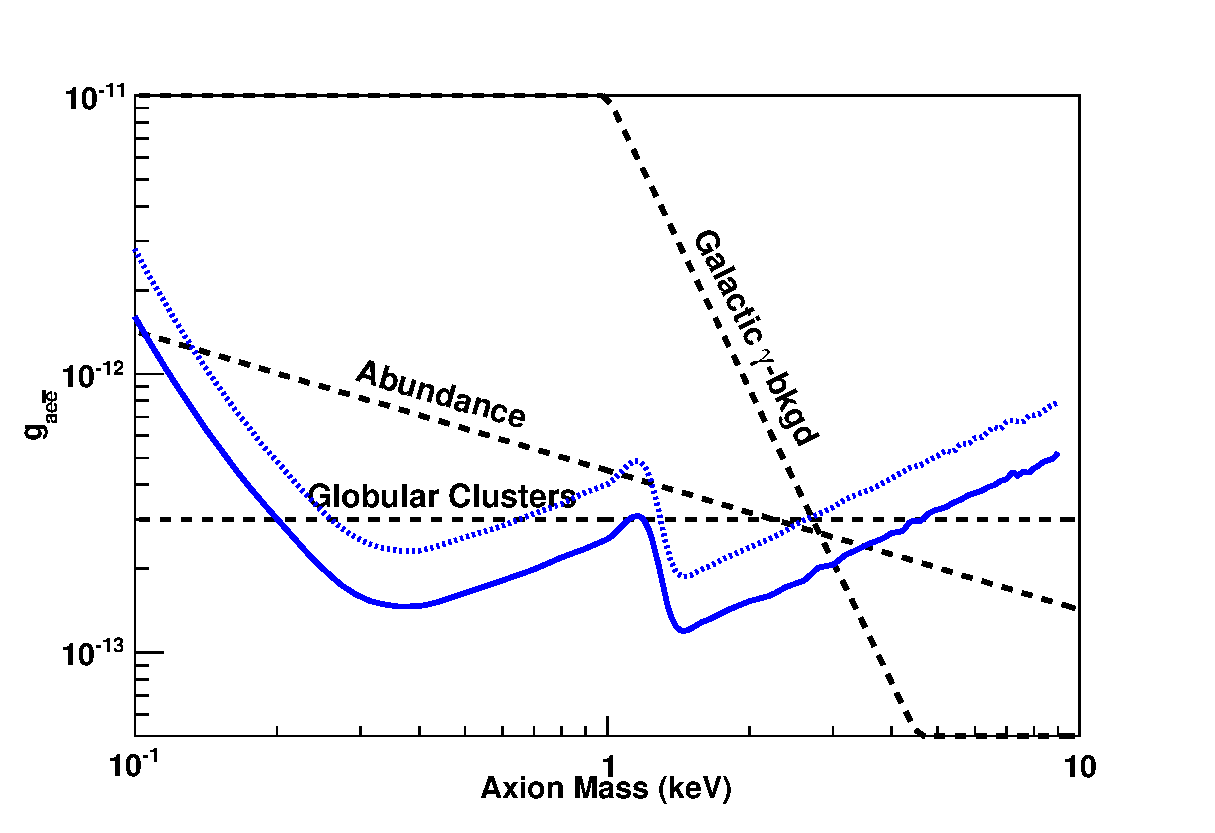
\includegraphics[width=0.9\textwidth]{MJAxionCompare}
				\caption{\MJ~\minmod~sensitivity at 90\% CL (blue curved lines, dotted 20~kg-yr exposure, solid 100~kg-yr exposure) to an axioelectric signal, 
				comparing to limits derived from astronomical observations including globular clusters~\cite{Raffelt95}, 
				axion abundance after the big bang, and constraints from observed galactic $\gamma$ 
				backgrounds~\cite{Pospelov:2008jk}.}
				\label{fig:MJSensitivityToHeavyAxionsCompare}
			\end{figure}							

	\section{Conclusions and Discussion}
	\label{sec:OtherLowEnergyConclusions}	
	
	The results of this chapter indicate the usefulness of \ppc~detectors for putting limits on dark matter, both for standard WIMP interactions as well as for more exotic interactions such as those from pseudoscalars.  The \MJ~\minmod~will play an important role in the dark matter field especially since it will provide an experimental platform for searching for dark matter particles other than WIMPs and should be competitive with limits from astronomical observation.  Of course, this chapter was unable to fully treat the rich landscape of available dark matter parameter space and some obvious candidates of study remain.  A spin-dependent WIMP interaction could be studied using the \minmod~since there exists one species of Ge with a non-zero nuclear spin:(\gerseventhree, $J=9/2^{+}$).  Since the relative content of this isotope in the detectors will be reduced by \gersevensix~enrichment, a comparison with detectors with natural \gerseventhree~abundance (7.7\%) could provide an opportunity for systematic studies.  The size of the detector array should also make it an excellent candidate for searching for a generic annual modulation signature of interactions with velocity dependence (e.g.~WIMP nuclear recoils).  As well, other more exotic hypothesis might already exist for which \MJ~could generate constraints, but those theories and analogous analyses of \MJ's sensitivity are left for the next thesis.
	
%This will be one of the more final discussions, but I can add to it later.  For now, focus on how these detectors can access different styles of dark matter because of their excellent energy resolution and threshold.  
